\documentclass[aspectratio=169]{beamer}
% \usepackage{pgfpages}
% \pgfpagesuselayout{4 on 1}[a4paper,landscape,border shrink=5mm]
\usepackage{tikz}
\usetikzlibrary{shapes, backgrounds, arrows, positioning}
\usepackage{pgfplots}
\usepackage{listings}
\usepackage[utf8,latin1]{inputenc}
\usepackage[style = apa, backend = biber, natbib = true]{biblatex}
\addbibresource{../../literature/lit.bib}

\makeatletter \def\newblock{\beamer@newblock} \makeatother  

\beamertemplatenavigationsymbolsempty
\setbeamertemplate{itemize items}[circle]
\setbeamertemplate{section in toc}[circle]
\mode<beamer>{\setbeamercolor{math text displayed}{fg=iwmgray}}
\setbeamercolor{block body}{bg=iwmorange!50!white}
\setbeamercolor{block title}{fg=white, bg=iwmorange}

% Definitions for biblatex
\setbeamercolor{bibliography entry note}{fg=iwmgray}
\setbeamercolor{bibliography entry author}{fg=iwmgray}
\setbeamertemplate{bibliography item}{}

\definecolor{iwmorange}{RGB}{255,105,0}
\definecolor{iwmgray}{RGB}{67,79,79}
\setbeamercolor{title}{fg=iwmorange}
\setbeamercolor{frametitle}{fg=iwmorange}
\setbeamercolor{structure}{fg=iwmorange}
\setbeamercolor{normal text}{fg=iwmgray}
\setbeamercolor{author}{fg=iwmgray}
\setbeamercolor{date}{fg=iwmgray}
\color{white}

\title{Pre/post measurements}
\author{Nora Wickelmaier}

\date{November 21, 2022}
%\date{Last modified: \today}

\newcommand{\vect}[1]{\mathbf{#1}}
\newcommand{\mat}[1]{\mathbf{#1}}
\newcommand{\gvect}[1]{\boldsymbol{#1}}
\newcommand{\gmat}[1]{\boldsymbol{#1}}

\lstset{language=R,%
  %backgroundcolor=\color{iwmgray!80!white},
  basicstyle=\ttfamily\color{iwmorange},
  frame=single,
  commentstyle=\slshape\color{black},
  keywordstyle=\bfseries\color{white},
  identifierstyle=\color{white},
  stringstyle=\color{green!85!black},
  numbers=none,%left,numberstyle=\tiny,
  basewidth={.5em, .4em},
  showstringspaces=false,
  emphstyle=\color{red!50!white}}

\lstdefinestyle{plain}{language=R,
  frame=none,
  basicstyle=\ttfamily\color{iwmorange},
  commentstyle=\slshape\color{iwmgray},
  keywordstyle=\bfseries\color{iwmgray},
  identifierstyle=\color{iwmgray},
  stringstyle=\color{iwmgray},
  numbers=none,
  basewidth={.5em, .4em},
  showstringspaces=false}

\pgfmathdeclarefunction{gauss}{2}{%
  \pgfmathparse{1/(#2*sqrt(2*pi))*exp(-((x-#1)^2)/(2*#2^2))}%
}

\AtBeginSection[]{
  \frame{
    \tableofcontents[sectionstyle=show/hide, subsectionstyle=show/show/hide]}}

\setbeamertemplate{headline}{
 \begin{beamercolorbox}{section in head}
   \vskip5pt\insertsectionnavigationhorizontal{\paperwidth}{}{}\vskip2pt
 \end{beamercolorbox}
}

\setbeamertemplate{footline}{\vskip-2pt\hfill\insertframenumber$\;$\vskip2pt}

\begin{document}

\begin{frame}{}
\thispagestyle{empty}
\titlepage
\end{frame}

\begin{frame}{Analysis of longitudinal data}
Advantages

\begin{itemize}
\item More power than cross sectional studies
\item Each subject is its own control person
\item Information about individual changes
\end{itemize}

Challenges
\begin{itemize}
\item Missing values
\item Predictors can change over time
\item In cross over designs: carry over effects
\end{itemize}
\end{frame}

\begin{frame}{Data schema}
\vfill
\begin{center}
\begin{tabular}{cccccc}
\hline
Person & Time      & Observation & \multicolumn{3}{c}{Covariates}\\\hline
1      & 1         & $y_{11}$    & $x_{111}$   & \dots & $x_{11p}$  \\
1      & 2         & $y_{12}$    & $x_{121}$   & \dots & $x_{12p}$  \\
.      & .         & .           & .           & \dots & .          \\
1      & $n_1$     & $y_{1n_1}$  & $x_{1n_11}$ & \dots & $x_{1n_1p}$\\
.      & .         & .           & .           & \dots & .          \\
.      & .         & .           & .           & \dots & .          \\
$N$    & 1         & $y_{N1}$    & $x_{N11}$   & \dots & $x_{N1p}$  \\
$N$    & 2         & $y_{N2}$    & $x_{N21}$   & \dots & $x_{N2p}$  \\
.      & .         & .           & .           & \dots & .          \\
$N$    & $n_N$     & $y_{Nn_N}$  & $x_{Nn_N1}$ & \dots & $x_{Nn_Np}$\\
\hline
\end{tabular}
\end{center}
\vfill
\end{frame}

\begin{frame}{Outline}
\tableofcontents
\end{frame}

\section[t test]{$t$ test}

\begin{frame}{$t$ test for dependent samples}
\begin{itemize}
  \item Straightforward analysis for two time points $n = 2$
  \item Written as linear model
    \begin{align*}
         d_i &= y_{i2} - y_{i1} \\
         d_i &= \beta_0 + \varepsilon_i \\
      y_{i2} &= \beta_0 + y_{i1} + \varepsilon_i
    \end{align*}
    with $\varepsilon_i \sim N(0, \sigma^2)$ i.i.d.
  \item Research question:\\
    Is there change between the first and second time point ($H_0\colon \beta_0 = 0$)?
  \item Which effects are not considered by this?
\end{itemize}
\end{frame}

\begin{frame}{Design}
\begin{itemize}
    \item At least two groups are observed before ($y_{i1}$) and after
      ($y_{i2}$) a treatment
        \begin{center}
        \begin{tikzpicture}
        \tikzstyle{every node}=[align=center]
        \node at (0.3, 3) (TG1) {TG1};
        \node at (0.3, 2.5) (TG2) {TG2};
        \node at (0.3, 2.1) (dots) {$\vdots$};
        \node at (0.3, 1.5) (CG) {CG};

        \node at (0, 1) (0) {};
        \node at (1.5, 1) [label=below:Baseline] (1) {};
        \node at (3, 1) (2) {$\cdots$};

        \node at (4.5, 1) [label=below:Treatment] (3) {};
        \node at (6, 1) (4) {$\cdots$};

        \node at (7.5, 1) [label=below:Follow-Up] (5) {};
        \node at (9, 1) (6) {};

        \foreach \x in {1.5, 4.5, 7.5} \draw[shift={(\x,1)}] (0pt,3pt) -- (0pt,-3pt);

        \draw               (0) -- (2);
        \draw               (2) -- (4);
        \draw[>=stealth,->] (4) -- (6) node[below] {$t$};
        \end{tikzpicture}
        \end{center}
      \item Research question:\\
      Do groups differ in the strength of their change?
\end{itemize}
\end{frame}

\begin{frame}{$t$ test for comparing two time points}
\begin{itemize}
  \item Consider for each person the change score $d_i = y_{i2} - y_{i1}$
    and the regression model
    \begin{align*}
         d_i &= \beta_0 + \varepsilon_i \\
      y_{i2} &= \beta_0 + y_{i1} + \varepsilon_i
    \end{align*}
    with $\varepsilon_i \sim N(0, \sigma^2)$ i.i.d.
  \item Interpretation:
    \begin{center}
    \begin{tabular}{ll}
    $\beta_0$ & average change score
    \end{tabular}
    \end{center}
  \item Hypothesis:\\
        Is there change between the first and second time point ($H_0\colon \beta_0 = 0$)?
  \item It is unclear if change is due to the treatment or just appeared
    over time
\end{itemize}
\end{frame}

\begin{frame}{$t$ test for comparing two time points}
\begin{center}
\begin{tikzpicture}[>=stealth, y=.6cm, x=.6cm, font=\small]
\draw[->] (0,0) -- coordinate (x axis mid) (10,0);
\draw[->] (0,0) -- coordinate (y axis mid) (0,10);
\node[below=0.5cm] at (x axis mid) {Pre-treatment score, $y_1$};
\node[rotate=90, above=0.5cm] at (y axis mid) {Post-treatment score, $y_2$};
%
\draw (0, 1) -- (8, 9);
\draw (6, 7) -- (7, 7) -- (7, 7.5) node [right] {$1$} -- (7, 8);
\draw[dashed] (0, 6) node [above right] {$\beta_0$} -- (5, 6) -- (5, 0) node [below] {$0$};
\end{tikzpicture}
\end{center}
\end{frame}

{\setbeamercolor{background canvas}{bg=iwmgray!80!white}

\begin{frame}[fragile]{$t$ test for comparing two time points}
\begin{lstlisting}
# simulate two dependent time points
cg <- MASS::mvrnorm(n=50, mu=c(10,10), Sigma=matrix(c(1,.9,.9,1), 2))
tg <- MASS::mvrnorm(n=50, mu=c(10,15), Sigma=matrix(c(1,.9,.9,1), 2))

sim <- as.data.frame(rbind(cg, tg))
names(sim) <- c("t1", "t2")

# add group variable
sim$group <- factor(rep(c("CG", "TG"), each=50))

# group means
aggregate(cbind(t1, t2) ~ group, sim, mean)
\end{lstlisting}
\end{frame}

\begin{frame}[fragile]{$t$ test for comparing two time points}
\begin{lstlisting}
# t test
t.test(sim$t2, sim$t1, paired=TRUE)

# add change score
sim$d <- sim$t2 - sim$t1

# linear model
lm1 <- lm(d ~ 1, sim)
lm2 <- lm(t2 ~ offset(t1), sim)

# visualization
plot(t2 ~ t1, sim)
abline(coef(lm2), 1)
\end{lstlisting}
\end{frame}

}


\begin{frame}{$t$ test of follow-up score of two groups}
\begin{itemize}
  \item In regression notation with $x_i = 1$, if $i$th person is part of
    the treatment group, and else $0$:
    \[
      y_{i2} = \beta_0 + \beta_1 \, x_i + \varepsilon_i
    \]
    with $\varepsilon_i \sim N(0, \sigma^2)$ i.i.d.
  \item Interpretation:
    \begin{center}
    \begin{tabular}{ll}
    $\beta_0$ & average follow-up score of reference group\\
    $\beta_1$ & effect of treatment group
    \end{tabular}
    \end{center}
  \item Hypothesis:\\
        Do groups differ at the second time point ($H_0\colon \beta_1 = 0$)?
  \item Since the baseline score is not considered, estimate of the change
    is biased
\end{itemize}
\end{frame}


\begin{frame}{$t$ test of follow-up score of two groups}
\begin{center}
\begin{tikzpicture}[>=stealth, y=.6cm, x=.6cm, font=\small]
\draw[->] (0,0) -- coordinate (x axis mid) (10,0);
\draw[->] (0,0) -- coordinate (y axis mid) (0,10);
\node[below=0.5cm] at (x axis mid) {Pre-treatment score, $y_1$};
\node[rotate=90, above=0.5cm] at (y axis mid) {Post-treatment score, $y_2$};
%
\draw (0, 5) node [above right] {$\beta_0 + \beta_1$} -- (9, 5) node [right] {TG};
\draw[dashed] (0, 3) node [above right] {$\beta_0$} -- (9, 3) node [right] {CG};
\end{tikzpicture}
\end{center}
\end{frame}

{\setbeamercolor{background canvas}{bg=iwmgray!80!white}

\begin{frame}[fragile]{$t$ test of follow-up score of two groups}
\begin{lstlisting}
# t test
t.test(t2 ~ group, sim, var.equal=TRUE)

# linear model
lm3 <- lm(t2 ~ group, sim)

# visualization
plot(t2 ~ t1, sim)
abline(h=cumsum(coef(lm3)))
\end{lstlisting}
\end{frame}

}

\section{Change score analysis}

\begin{frame}{Change score analysis}
\begin{itemize}
  \item Regression model
    \begin{align*}
                  d_i &= \beta_0 + \beta_1 \, x_i + \varepsilon_i \\
      y_{i2} - y_{i1} &= \beta_0 + \beta_1 \, x_i + \varepsilon_i \\
               y_{i2} &= \beta_0 + y_{i1} + \beta_1 \, x_i + \varepsilon_i
    \end{align*}
    with $\varepsilon_i \sim N(0, \sigma^2)$ i.i.d.
  \item Interpretation:
    \begin{tabular}{lp{10cm}}
    $\beta_0$ & average change score for reference group\\
    $\beta_1$ & difference to $\beta_0$ in treatment group
    \end{tabular}
  \item Hypothesis:
    \begin{itemize}
        \item Is there change in the reference group ($H_0\colon \beta_0 = 0$)?
        \item Does the change differ between groups ($H_0\colon \beta_1 =0$)?
    \end{itemize}
\end{itemize}
\end{frame}


\begin{frame}{Change score analysis}
\begin{center}
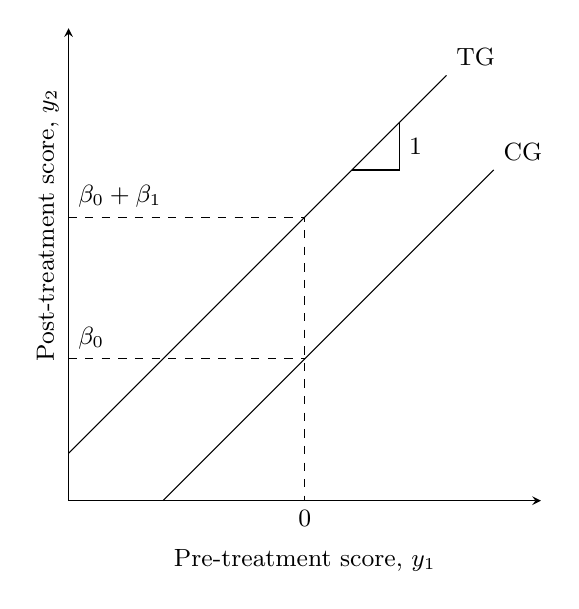
\begin{tikzpicture}[>=stealth, y=.6cm, x=.6cm, font=\small]
\draw[->] (0,0) -- coordinate (x axis mid) (10,0);
\draw[->] (0,0) -- coordinate (y axis mid) (0,10);
\node[below=0.5cm] at (x axis mid) {Pre-treatment score, $y_1$};
\node[rotate=90, above=0.5cm] at (y axis mid) {Post-treatment score, $y_2$};
%
\draw (0, 1) -- (8, 9) node [above right] {TG};
\draw (6, 7) -- (7, 7) -- (7, 7.5) node [right] {$1$} -- (7, 8);
\draw[dashed] (0, 6) node [above right] {$\beta_0 + \beta_1$} -- (5, 6) -- (5, 0) node [below] {$0$};
\draw (2, 0) -- (9, 7) node [above right] {CG};
\draw[dashed] (0, 3) node [above right] {$\beta_0$} -- (5, 3);
\end{tikzpicture}
\end{center}
\end{frame}

{\setbeamercolor{background canvas}{bg=iwmgray!80!white}

\begin{frame}[fragile]{Change score analysis}
\begin{lstlisting}
# regression model
lm4 <- lm(t2 ~ offset(t1) + group, sim)

# visualization
plot(t2 ~ t1, sim)
abline(coef(lm4)[1], 1)
abline(coef(lm4)[1] + coef(lm4)[2], 1)
\end{lstlisting}
\end{frame}

}

\begin{frame}{Regression to the mean}
\begin{itemize}
  \item Change score analysis is based on the often too restrictive
    assumption that the follow-up score depends on the baseline score with
    a slope of $1$
  \item Often baseline scores are negatively correlated with the change
    scores:\\
    Persons with low (bad) scores improve more than persons with high scores
  \item This regression to the mean lets us expect a slope of $< 1$ which
    has to be estimated from the data
\end{itemize}
\end{frame}

\section[ANCOVA]{Analysis of covariance}

\begin{frame}{Analysis of covariance (ANCOVA)}
\begin{itemize}
  \item Regression model
    \[
      y_{i2} = \beta_0 + \beta_1 \, y_{i1} + \beta_2 \, x_i + \varepsilon_i
    \]
    with $\varepsilon_i \sim N(0, \sigma^2)$ i.i.d.
  \item Interpretation:
    \begin{tabular}{lp{10cm}}
    $\beta_0$ & average follow-up score in the reference group for $y_{i1} = 0$\\
    $\beta_1$ & effect of baseline score\\
    $\beta_2$ & difference to follow-up score in the treatment group
    \end{tabular}
  \item Hypothesis:
    \begin{itemize}
        \item Is there a relationship between baseline and follow-up score ($H_0\colon \beta_1 = 0$)?
        \item Do the follow-up scores in the groups differ for persons with
          identical baseline scores ($H_0\colon \beta_2 = 0$)?
    \end{itemize}
\end{itemize}
\end{frame}


\begin{frame}{Analysis of covariance (ANCOVA)}
\begin{center}
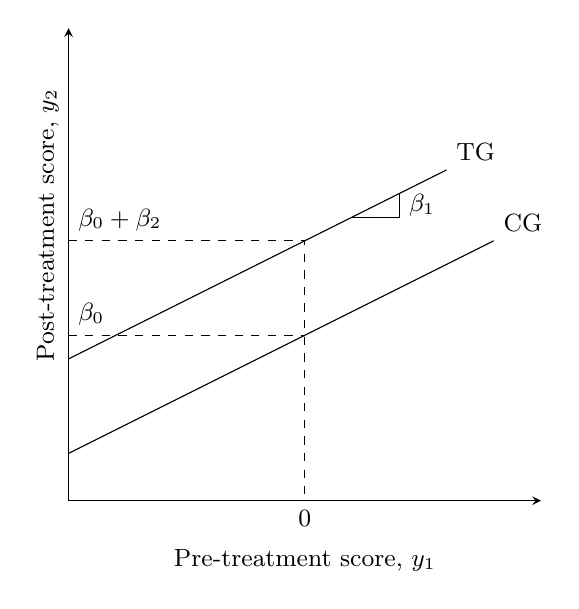
\begin{tikzpicture}[>=stealth, y=.6cm, x=.6cm, font=\small]
\draw[->] (0,0) -- coordinate (x axis mid) (10,0);
\draw[->] (0,0) -- coordinate (y axis mid) (0,10);
\node[below=0.5cm] at (x axis mid) {Pre-treatment score, $y_1$};
\node[rotate=90, above=0.5cm] at (y axis mid) {Post-treatment score, $y_2$};
%
\draw (0, 3) -- (8, 7) node [above right] {TG};
\draw (6, 6) -- (7, 6) -- (7, 6.25) node [right] {$\beta_1$} -- (7, 6.5);
%
\draw[dashed] (0, 5.5) node [above right] {$\beta_0 + \beta_2$} -- (5, 5.5) -- (5, 0) node [below] {$0$};
%
\draw (0, 1) -- (9, 5.5) node [above right] {CG};
\draw[dashed] (0, 3.5) node [above right] {$\beta_0$} -- (5, 3.5);
\end{tikzpicture}
\end{center}
\end{frame}


\begin{frame}{Adjusted means}
\begin{itemize}
  \item With an ANCOVA model we can predict average follow-up scores for
    persons with the same baseline score
  \item For example, we get
    \[
      \hat{y}_{i2} = \hat{\beta}_0 + \hat{\beta}_1 \, \bar{y}_1 +
                     \hat{\beta}_2 \, x_i
    \]
    for an average baseline score $\bar{y}_1$
\item These conditional means are sometimes called (baseline) adjusted
  means
\end{itemize}
\end{frame}

{\setbeamercolor{background canvas}{bg=iwmgray!80!white}

\begin{frame}[fragile]{Analysis of covariance (ANCOVA)}
\begin{lstlisting}
# ancova
lm5 <- lm(t2 ~ t1 + group, sim)

# adjusted means
predict(lm5, newdat=data.frame(t1=mean(sim$t1), group=c("CG", "TG")))

# ancova with change score
lm5a <- lm(d ~ t1 + group, sim)

# visualization
plot(t2 ~ t1, sim)
abline(coef(lm5)[1], coef(lm5)[2])
abline(coef(lm5)[1] + coef(lm5)[3], coef(lm5)[2])
\end{lstlisting}
\end{frame}

}

\begin{frame}{Analysis of covariance with change score}
\begin{itemize}
  \item Regression model
    \begin{align*}
                  d_i &= \beta_0 + \beta_1 \, y_{i1} + \beta_2 \, x_i + \varepsilon_i \\
      y_{i2} - y_{i1} &= \beta_0 + \beta_1 \, y_{i1} + \beta_2 \, x_i + \varepsilon_i \\
               y_{i2} &= \beta_0 + (1 + \beta_1) \, y_{i1} + \beta_2 \, x_i + \varepsilon_i
    \end{align*}
  \item For testing the difference of change in the groups ($\beta_2$) it
    is irrelevant if the dependent variable is the follow-up score or the
    change score
  \vfill
\end{itemize}
\end{frame}

\begin{frame}{Different slopes for groups}
\begin{itemize}
  \item Regression model
    \[
      y_{i2} = \beta_0 + \beta_1 \, y_{i1} + \beta_2 \, x_i +
               \beta_3 \, (y_{i1} \cdot x_i) + \varepsilon_i
    \]
    with $\varepsilon_i \sim N(0, \sigma^2)$ i.i.d.
  \item Interpretation:
    \begin{tabular}{lp{10cm}}
    $\beta_0$ & average follow-up score in reference group for $y_{i1} = 0$\\
    $\beta_1$ & effect of baseline score\\
    $\beta_2$ & difference to follow-up score in treatment group\\
    $\beta_3$ & difference between slopes in reference and treatment groups
    \end{tabular}
  \item Hypothesis:\\
        Does effect of baseline score depend on group ($H_0\colon \beta_3 = 0$)?
  \item Interpretation of adjusted means idenpendently of baseline score
    implies $\beta_3 = 0$
\end{itemize}
\end{frame}


\begin{frame}{Interaction between baseline score and group}
\begin{center}
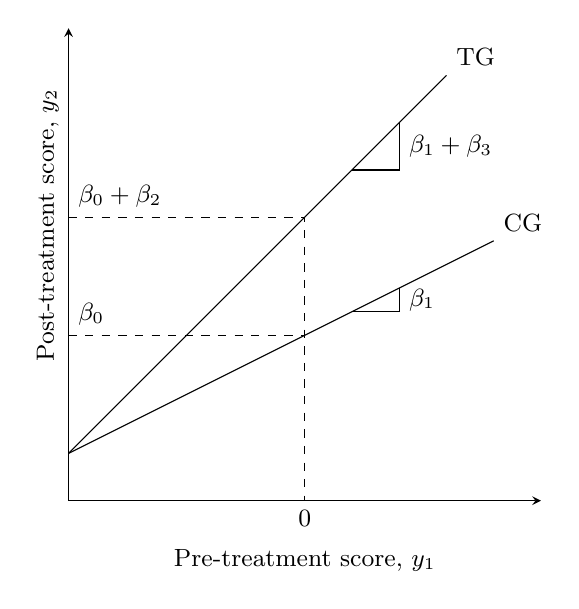
\begin{tikzpicture}[>=stealth, y=.6cm, x=.6cm, font=\small]
\draw[->] (0,0) -- coordinate (x axis mid) (10,0);
\draw[->] (0,0) -- coordinate (y axis mid) (0,10);
\node[below=0.5cm] at (x axis mid) {Pre-treatment score, $y_1$};
\node[rotate=90, above=0.5cm] at (y axis mid) {Post-treatment score, $y_2$};
%
\draw (0, 1) -- (8, 9) node [above right] {TG};
\draw (6, 7) -- (7, 7) -- (7, 7.5) node [right] {$\beta_1 + \beta_3$} -- (7, 8);
\draw[dashed] (0, 6) node [above right] {$\beta_0 + \beta_2$} -- (5, 6) -- (5, 0) node [below] {$0$};
%
\draw (0, 1) -- (9, 5.5) node [above right] {CG};
\draw (6, 4) -- (7, 4) -- (7, 4.25) node [right] {$\beta_1$} -- (7, 4.5);
\draw[dashed] (0, 3.5) node [above right] {$\beta_0$} -- (5, 3.5);
\end{tikzpicture}
\end{center}
\end{frame}

{\setbeamercolor{background canvas}{bg=iwmgray!80!white}

\begin{frame}[fragile]{Interaction between baseline score and group}
\begin{lstlisting}
# regression model with interaction
lm6 <- lm(t2 ~ t1*group, sim)

# visualization
plot(t2 ~ t1, sim)
abline(coef(lm6)[1], coef(lm6)[2])
abline(coef(lm6)[1] + coef(lm6)[3], coef(lm6)[2] + coef(lm6)[4])

# models are nested
anova(lm4, lm5, lm6)
\end{lstlisting}
\end{frame}

}

\section[Example]{Example: Acupuncture for shoulder pain}

\begin{frame}{Example: Acupuncture for shoulder pain}
\begin{itemize}
  \item \citet{Kleinhenz1999} investigated the effect of acupuncture on
    the improvement of mobility for 52 patients with shoulder pain
  \item Patients were randomly assigned to two groups (placebo vs.\
    acupuncture)
  \item Before and after the treatment a mobility score was measured
  \item \citet{VickersAltman2001} show advantages of an analysis of
    covariance compared to other methods based on these data
\end{itemize}
\end{frame}


\begin{frame}{Acupuncture: Follow-up analysis}
\begin{columns}[T]
\begin{column}{5.5cm}
  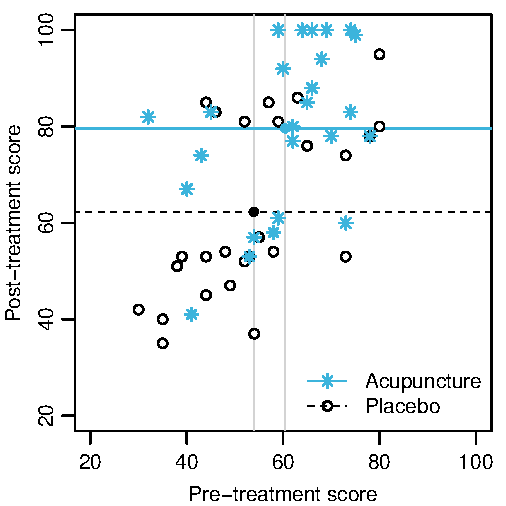
\includegraphics[width=5.5cm]{../figures/acu-fwup}
\end{column}
%
\begin{column}{5.5cm}
  \vspace*{1em}\small
  \begin{tabular}{lrrr}
  \hline
             &  Pla &  Acu & Diff \\ \hline
  Baseline   & 53.9 & 60.4 &  6.5 \\
  Follow-up  & 62.3 & 79.6 & 17.3 \\
  Change sc. &  8.4 & 19.2 & 10.8 \\
  ANCOVA     &      &      & 12.7 \\ \hline
  \end{tabular}
\begin{align*}
         y_{i2} &= \beta_0 + \beta_1 \, x_i + \varepsilon_i \\
  \hat{\beta}_1 &= 17.3, 0.95\text{-CI: } (7.5, 27.1)
\end{align*}
\end{column}
\end{columns}
\end{frame}


\begin{frame}{Acupuncture: Change score analysis}
\begin{columns}[T]
\begin{column}{5.5cm}
  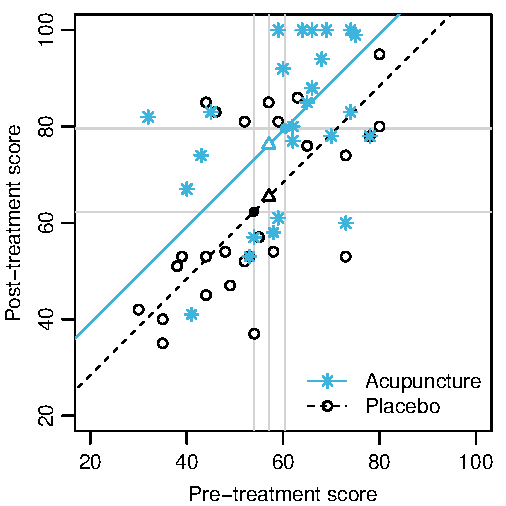
\includegraphics[width=5.5cm]{../figures/acu-chng}
\end{column}
%
\begin{column}{5.5cm}
  \vspace*{1em}\small
  \begin{tabular}{lrrr}
  \hline
             &  Pla &  Acu & Diff \\ \hline
  Baseline   & 53.9 & 60.4 &  6.5 \\
  Follow-up  & 62.3 & 79.6 & 17.3 \\
  Change sc. &  8.4 & 19.2 & 10.8 \\
  ANCOVA     &      &      & 12.7 \\ \hline
  \end{tabular}
\begin{align*}
         y_{i2} &= \beta_0 + y_{i1} + \beta_1 \, x_i + \varepsilon_i \\
  \hat{\beta}_1 &= 10.8 \; (2.3, 19.4)
\end{align*}
\end{column}
\end{columns}
\end{frame}


\begin{frame}{Acupuncture: ANCOVA}
\begin{columns}[T]
\begin{column}{5.5cm}
  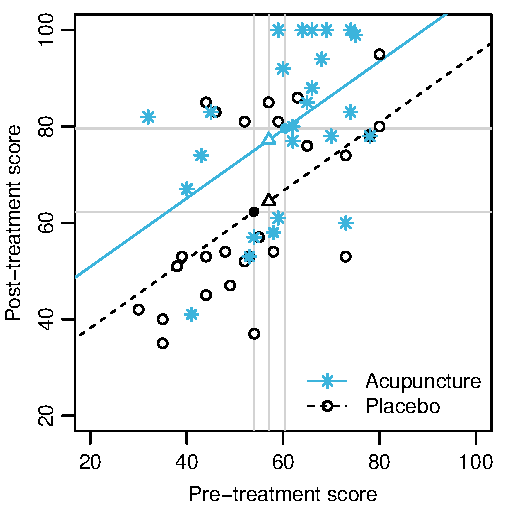
\includegraphics[width=5.5cm]{../figures/acu-anco}
\end{column}
%
\begin{column}{5.5cm}
  \vspace*{1em}\small
  \begin{tabular}{lrrr}
  \hline
             &  Pla &  Acu & Diff \\ \hline
  Baseline   & 53.9 & 60.4 &  6.5 \\
  Follow-up  & 62.3 & 79.6 & 17.3 \\
  Change sc. &  8.4 & 19.2 & 10.8 \\
  ANCOVA     &      &      & 12.7 \\ \hline
  \end{tabular}
\begin{align*}
         y_{i2} &= \beta_0 + \beta_1 \, y_{i1} + \beta_2 \, x_i +
                    \varepsilon_i \\
  \hat{\beta}_2 &= 12.7 \; (4.1, 21.3)
\end{align*}
\end{column}
\end{columns}
\end{frame}

{\setbeamercolor{background canvas}{bg=iwmgray!80!white}

\begin{frame}[fragile]{Example: Acupuncture for shoulder pain}
\begin{lstlisting}
# read data
dat <- read.table("kleinhenz.txt", header=TRUE)
dat$grp <- factor(dat$grp, levels=c("plac", "acu"))

# follow-up analysis
m1 <- lm(post ~ grp, dat)
summary(m1)
confint(m1)

# change score analysis
m2 <- lm(post ~ offset(pre) + grp, dat)

# ancova
m3 <- lm(post ~ pre + grp, dat)
\end{lstlisting}
\end{frame}

\begin{frame}[fragile]{Example: Acupuncture for shoulder pain}
\begin{lstlisting}
# testing if slopes differ
m4 <- lm(post ~ pre*grp, dat)
anova(m3, m4)

# adjusted means
predict(m3, data.frame(pre=mean(dat$pre), grp=c("plac", "acu")))

# visualization
plot(post ~ pre, dat, xlim=c(20,100), ylim=c(20,100))
abline(coef(m3)[1], coef(m3)[2])
abline(coef(m3)[1] + coef(m3)[3], coef(m3)[2])
\end{lstlisting}
\end{frame}

% \begin{frame}[fragile]{R-Demo}{}
% %
% Grafische Darstellung
% \begin{lstlisting}
% omean <- tapply(dat$post, dat$grp, mean)
% pmean <- predict(m3, data.frame(pre=mean(dat$pre),
%                  grp=c("plac", "acu")))
% par(mai=c(.6, .6, .1, .1), mgp=c(2, .7, 0))
% plot(post ~ pre, dat, type="n", xlim=c(20,100), ylim=c(20,100),
%      xlab="Pre-treatment score", ylab="Post-treatment score")
% abline(h=c(pmean, omean), v=c(mean(dat$pre),
%                  tapply(dat$pre, dat$grp, mean)), col="lightgray")
% xval <- 1:100
% lines(predict(m3, data.frame(pre=xval, grp="plac")) ~ xval, lty=2)
% lines(predict(m3, data.frame(pre=xval, grp="acu" )) ~ xval)
% points(post ~ pre, dat[dat$grp == "plac", ], pch=21, bg="white")
% points(post ~ pre, dat[dat$grp == "acu", ],  pch=8)
% points(omean ~ tapply(pre, grp, mean), dat, pch=16)
% points(pmean ~ rep(mean(pre), 2), dat, pch=24, bg="white")
% legend("bottomright", c("Acupuncture", "Placebo"),
%        pch=c(8, 1), lty=1:2, bty="n")
% \end{lstlisting}
% %\vspace*{-0.5em}
% %
% \end{frame}

}


\begin{frame}{Summary}
\begin{itemize}
  \item We considered the basic case when several groups are observed at
    two time points (baseline and follow-up)
  \item Analysis of these kind of data considers the difference
    \[
        d_i = y_{i2} - y_{i1}
    \]
    or the adjusted follow-up scores which are considered to be independent
  \item Analysis of covariance
  \begin{itemize}
    \item has the highest power to detect differences for average change
      compared to the other methods
    \item must be cautiously interpreted when groups are not randomly
      assigned
  \end{itemize}
\end{itemize}
\end{frame}

\appendix

\section{Repeated measures ANOVA}

\begin{frame}{Repeated measures ANOVA}
\begin{itemize}
  \item Regression notation with indicator variable for time ($t_{i1} = 0$,
    $t_{i2} = 1$) and\\ group ($x_i$)
    \[
      y_{ij} = \beta_0 + \beta_1 \, t_{ij} + \beta_2 \, x_i +
               \beta_3 \, (t_{ij} \cdot x_i) + \upsilon_i + \varepsilon_{ij}
    \]
    with $\upsilon_i \sim N(0, \sigma^2_\upsilon)$ and $\varepsilon_{ij}
    \sim N(0, \sigma^2)$
  \item Interpretation:
    \begin{center}
    \begin{tabular}{lp{10cm}}
    $\beta_0$ & mean baseline value in reference group\\
    $\beta_1$ & time effect (slope) in reference group\\
    $\beta_2$ & effect of treatment group\\
    $\beta_3$ & effect on the slope of treatment group
    \end{tabular}
    \end{center}
\end{itemize}
\end{frame}

\begin{frame}{Repeated measures ANOVA}
\begin{center}
\begin{tikzpicture}[>=stealth, y=.6cm, x=.6cm, font=\small]
\draw[->] (0,0) -- coordinate (x axis mid) (10,0);
\draw[->] (0,0) -- coordinate (y axis mid) (0,10);
\node[below=0.5cm] at (x axis mid) {Time, $t$};
\node[rotate=90, above=0.5cm] at (y axis mid) {Response, $y$};
%
\draw (3, 4) -- (7, 8) node [above right] {TG};
\draw (4.5, 5.5) -- (5.5, 5.5) -- (5.5, 6) node [right] {$\beta_1 + \beta_3$} -- (5.5, 6.5);
\draw[dashed] (0, 4) node [above right] {$\beta_0 + \beta_2$} -- (3, 4);
%
\draw (3, 2) -- (7, 4) node [above right] {CG};
\draw (4.5, 2.75) -- (5.5, 2.75) -- (5.5, 3.0) node [right] {$\beta_1$} -- (5.5, 3.25);
\draw[dashed] (0, 2) node [above right] {$\beta_0$} -- (3, 2);
%
\draw plot[only marks, mark size=1pt, mark=*]
    coordinates {(3, 4) (7, 8) (3, 2) (7, 4)};
\draw (3, 0.1) -- (3, 0) node [below] {$0$};
\draw (7, 0.1) -- (7, 0) node [below] {$1$};
\end{tikzpicture}
\end{center}
\end{frame}

\begin{frame}{Repeated measures ANOVA}
\begin{itemize}
  \item For the two groups with $j = 1, 2$, we get
    \begin{align*}
      y_{i1} &= \beta_0 + \beta_2 \, x_i + \upsilon_i + \varepsilon_{i1}\\
      y_{i2} &= \beta_0 + \beta_1 + \beta_2 \, x_i + \beta_3 \, x_i + \upsilon_i + \varepsilon_{i2}
    \end{align*}
  \vspace{-.4cm}
  \item For the change score, we then get
    \[
      y_{i2} - y_{i1} = \beta_1 + \beta_3 \, x_i + (\varepsilon_{i2} - \varepsilon_{i1})
    \]
  \vspace{-.4cm}
  \item Since $\varepsilon_{ij}$ are independent, this results in the
    equation for the change score analysis
    \[
        y_{i2} - y_{i1} = \beta_1 + \beta_3 \, x_i + \varepsilon_{i}
    \]
    with
    \[
        \varepsilon_i = \varepsilon_{i2} - \varepsilon_{i1} \sim N(0, \sigma_d^2 = 2 \sigma^2)
    \]
\end{itemize}
  \vspace{-.3cm}
  $\to$ ANOVA for two time points is equivalent to change score analysis!
\end{frame}

{\setbeamercolor{background canvas}{bg=iwmgray!80!white}


\begin{frame}[fragile]{Example: Acupuncture for shoulder pain}
\begin{lstlisting}
# Read data
dat <- read.table("kleinhenz.txt", header=TRUE)
dat$grp <- factor(dat$grp, levels=c("plac", "acu"))

# Change score analysis
m1 <- lm(post ~ offset(pre) + grp, dat)
# Repeated-measures ANOVA
datl <- reshape(dat, direction="long", varying=list(1:2), v.names="score")
datl$time <- factor(datl$time, levels=1:2, labels=c("pre", "post"))
m2 <- lmer(score ~ grp*time + (1 | id), datl)

# Compare residual variances
sigma(m1)^2
2 * sigma(m2)^2
\end{lstlisting}
\end{frame}

}


% {\setbeamercolor{background canvas}{bg=iwmgray!80!white}
% 
% \begin{frame}[fragile]{}
%   \begin{lstlisting}
%   ##
%   \end{lstlisting}
% \end{frame}
% 
% }
% 
% \begin{frame}[fragile]{}
%   \begin{block}{Exercise}
%     \begin{itemize}
%       \item 
%     \end{itemize}
%   \end{block}
% \end{frame}

%\begin{frame}[allowframebreaks]{References}
\begin{frame}{References}
  \printbibliography
  \vfill
\end{frame}

\end{document}

